\section{Data Collection}

We have collected data from FDIC website with a list of failed banks since Oct
2000, which contains acquiring institutions, and another list of failed banks
since the establishment of FDIC.

We joined the two tables based on their CERT number, which is a primary key of
the tables. We filtered out any items that has N/A in the estimated loss
column, which are all in 2017. Now we have data from Oct 2000 to Dec 2016.

We also want to get the geographic coordinates (longitutde and latitude) of
the headquarters of the failed banks. We used a site called www.latlong.net.
The site has a input box where one can enter the name of a location and a
button ``find'', which loads the latitude and longitude into the other two
input boxes when clicked. This website is awesome except that the api are
hidden in a complex and lengthy JavaScript. Instead of trying to decipher the
JavaScript code, we wrote a script to emulate input and click to fetch the
coordinates for a list of locations. The script is in data/latlong.net.js,
where the first part is used to load jQuery and has to be run first
separately. After a few seconds, we can paste the remaining part of the script
into the console in Chrome. Then we set the city\_names global variable to a
list of locations we want to get coordinates for and invoke start\_first().
After a while, the results global variable is populated with a list of triple
of location name, latitude and longitude.

A note to the script: there has to be a wait after both input to the location
name box and clicking the find button. I don't know if this is due to the lag
of my system or network issue or google map needs more time to load or their
bugs. Now I set both waits at 5 seconds. On my own laptop, this allows me to
fetch more than 300 locations in a row without any error. In case an error
occurs, an alert dialog (which is part of the website's design, not mine),
will pop up saying invalid location. When this happens, the current location
in the input box has better to be recorded so that we can come back to do it
again (manually of course). The remainder of the script will typically run as
usual. From my personal experience, when the number of location gets near 400,
the error starts to pop up every 1 or 2 locations. I had to manually correct
about 40 locations.

We then joined the coordinates with the data. Some of the data are in Puerto
Rico, which cannot be correctly displayed by d3.geoAlbersUsa(). We simply
filtered out those records.

\newpage

\section{Screenshot before milestone (Nov 10, 2017)}

\begin{figure}[!h]
    \centering
    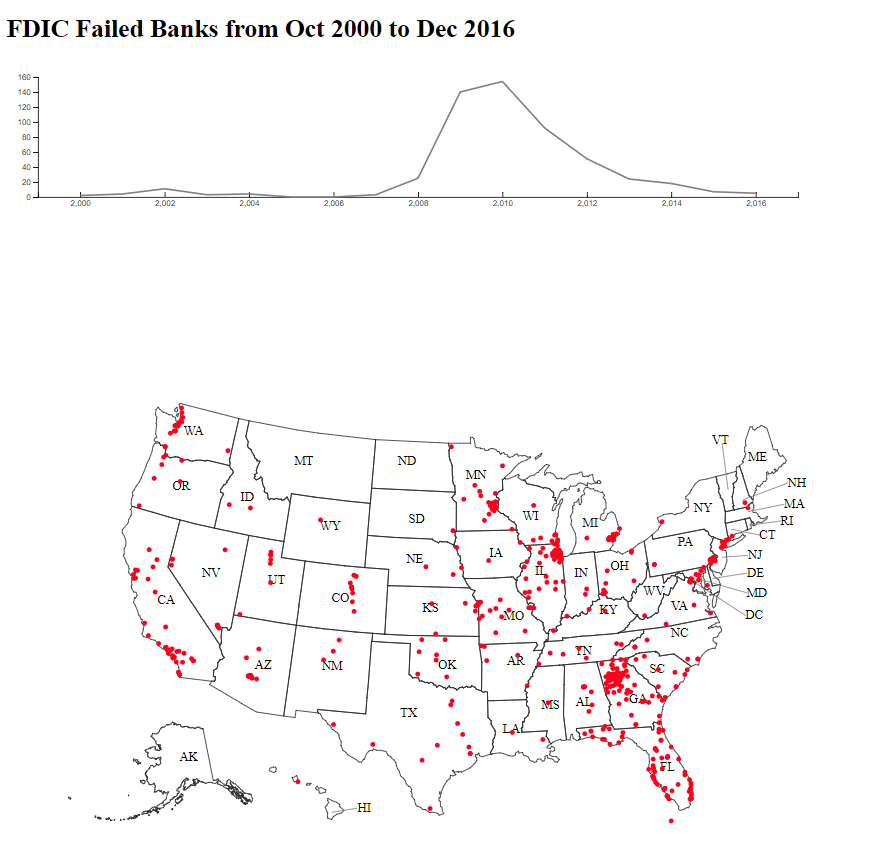
\includegraphics[width=\textwidth]{fig/Nov10}
    \caption{A screenshot for the milestone as of November 10}
    \label{fig:milestone}
\end{figure}

Now, this is what we have (see Figure \ref{fig:milestone}) as of the milestone
(Nov 10, 2017). We have the line chart and the map set up with the bar chart
yet to complete. 

The line chart still doesn't have a drop-down list to select
the y-axis, which is currently the number of failed banks in a year. We plan
to add a dots to the line chart so that a user can easily select one or some
of the years. We also plan to add tooltips to each dot so that the exact
number is easy to read, as some of them are quite small compared to those of
2008-2010.

The map hasn't been linked to the line chart and only plots the full dataset.
As shown in the figure, some areas has dense population of failed banks,
making it hard to use tooltip to show the details. And some of the banks are
in the same city (e.g., surprisingly 19 in Chicago, IL, 10 in Atlanta, GA,
while New York City only has 2), which also makes tooltip infeasible. Instead
of tooltips, we plan to use 2D brush to select a range of banks. And we'll
show a list of those banks. The user can click on one of them to expand the
detailed information about it on a separate box.

Hopefully, our work will have a functioning line chart and map by the next
week.

\newpage

\section{Line Chart}

\begin{figure}[!h]
    \centering
    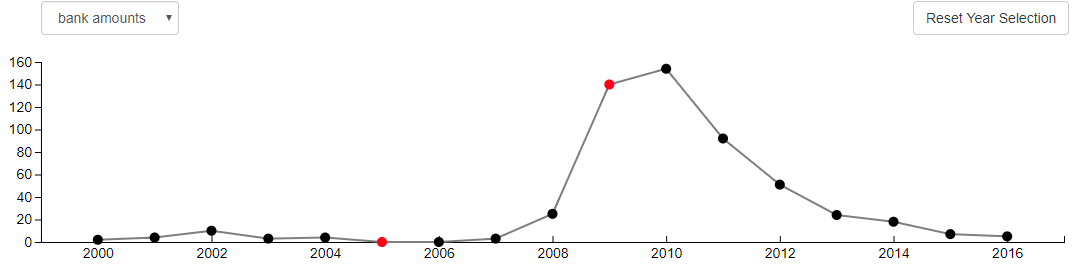
\includegraphics[width=0.9\textwidth]{fig/linechart}
    \caption{The line chart}
    \label{fig:linechart}
\end{figure}

The line chart (Figure~\ref{fig:linechart}) serves as our primary view
which allows the user to have an overview of the temporal aggregates of the
failed banks. This part is primarily implemented by Ya. She first implemented
a line chart that features two axises with the y-axis configurable via a
drop-down box, a line with scatter points that represents each years' data on
it. The user can select/de-select one or multiple years to change the data
shown in the bar chart as well as the map. If none is selected, all years are
assumed to be selected. Compared to the 1-D brushing used in the Brazil world
cup homework, it has a much better flexibility in that the selected years are
not necessarily consecutive. It, however, is hard for the user to start over
with the selection. In order to overcome that problem, we introduced a "reset
year selection" button that allows the user the clear all the selections.

\newpage

\section{Map}

\begin{figure}[!h]
    \centering
    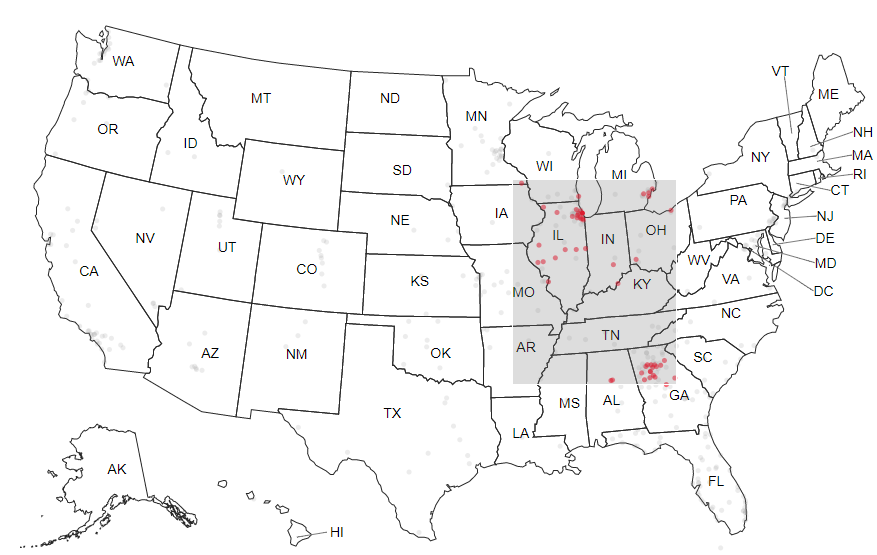
\includegraphics[width=0.9\textwidth]{fig/map}
    \caption{The map}
    \label{fig:map}
\end{figure}

The map (Figure~\ref{fig:map}) allows the user to freely browse and search for
the spatial distribution and the details of the failed banks. This part is
primarily implemented by Zhuoyue. We derived the map from the map data in the
course material in lecture 9. As we mentioned before, we crawled the
geo-coordinates of all the states the banks' cities from www.latlong.net. We
immediately identified two challenges. First, the states on the northeast as
well as Hawaii have small areas on the map, so we need to use an alternate
coordinates for their names and certain states' coordinates are a bit off. We
manually fixed the locations of them in the data. Second, certain cities have
multiple failed banks (e.g. 18 in Chicago). Instead of plotting a point for
each for bank, we grouped the banks by their cities, and plot the cities
instead. We have a 2D brushing on the map so a user can select a rectangular
region. If he/she is interested in a particular state or several adjacent
states, 2D brushing is a good solution for such selection. We did not
investigate multi-selection but it might be interesting to try to implement
that if time permits. If any of the bank in the city is in the selection
(according to the years in the line chart, the 2D brush on the map and the
text search we will describe later), the point for that city is shown.

Initially, we simply hide those points that have no banks in the selection
while the others are shown in red with no opacity. We later found out that
setting the opacity of each point to some range can better represent the
density of banks. The points not in the selection can be set to a very low
opacity so that they can still be seen but will not attract unnecessary
attention from the user.

\begin{figure}[!h]
    \centering
    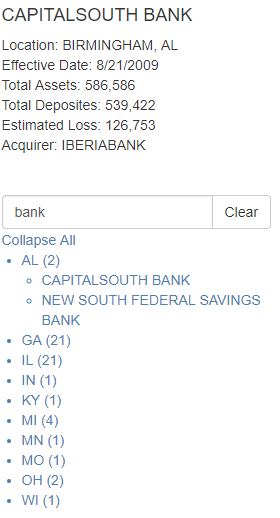
\includegraphics{fig/searchbox}
    \caption{The search box area}
    \label{fig:searchbox}
\end{figure}
Finally, we have a search box and a list of banks in the selection
(Figure~\ref{fig:searchbox}). The text in the search box (regardless in lower
case or upper case), are searched in the names of the failed banks. A bank is
said to be in the selection, if its effective year is selected in the line
chart and its name contains the substring in the search box. In addition to
being highlighted on the map in red, the banks are listed in the unordered
list under the search box, grouped by states, where the states can be expanded
or collapsed. If a bank in the list is clicked, its details are shown above
the search box.


\newpage

\section{Bar chart}

\begin{figure}[!h]
    \centering
    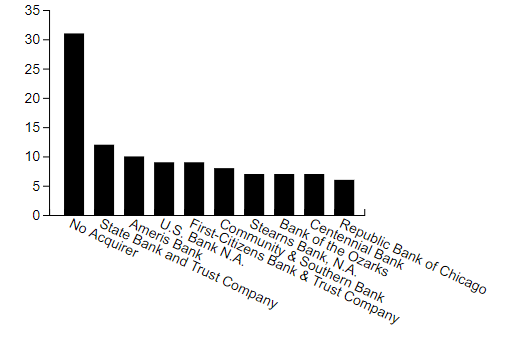
\includegraphics{fig/barchart}
    \caption{The bar chart}
    \label{fig:barchart}
\end{figure}

The bar chart (Figure~\ref{fig:barchart}) mainly show the top acquirers of the
failed banks. This part is primarily handled by Ya and Zhuoyue also have
significant changes to it. Since no FDIC insured funds have ever
been lost, it is interesting to us to see how are the failed banks are
absorbed by different entities. We limited them to at most the largest 10 such
entity according to the y-axis as defined in the line chart so that we do not
run out of display space. An challenge is to properly display the name of the
acquiring institutions without get cut off. We find that rotating 30 degrees
and setting the font size to 14px gives us the best result in terms of space
compactness and readability.

Initially, we designed the bar chart to only reflect the year selection but we
later found that it is quite intuitive when a user is also selecting regions
on the map as well as filtering the banks using the search box. So we changed
the bar chart to honor all the three selections. A nice side effect of that is
we can easily find the top acquirers in a specific region.

A down-side of a single view is its inability to allow comparison between
different selections. An alternate approach would be allowing creating
multiple views according to different selections, which, however, we do not
have enoght time to explore.


\newpage
\section{Summary}

\begin{figure}[!th]
    \centering
    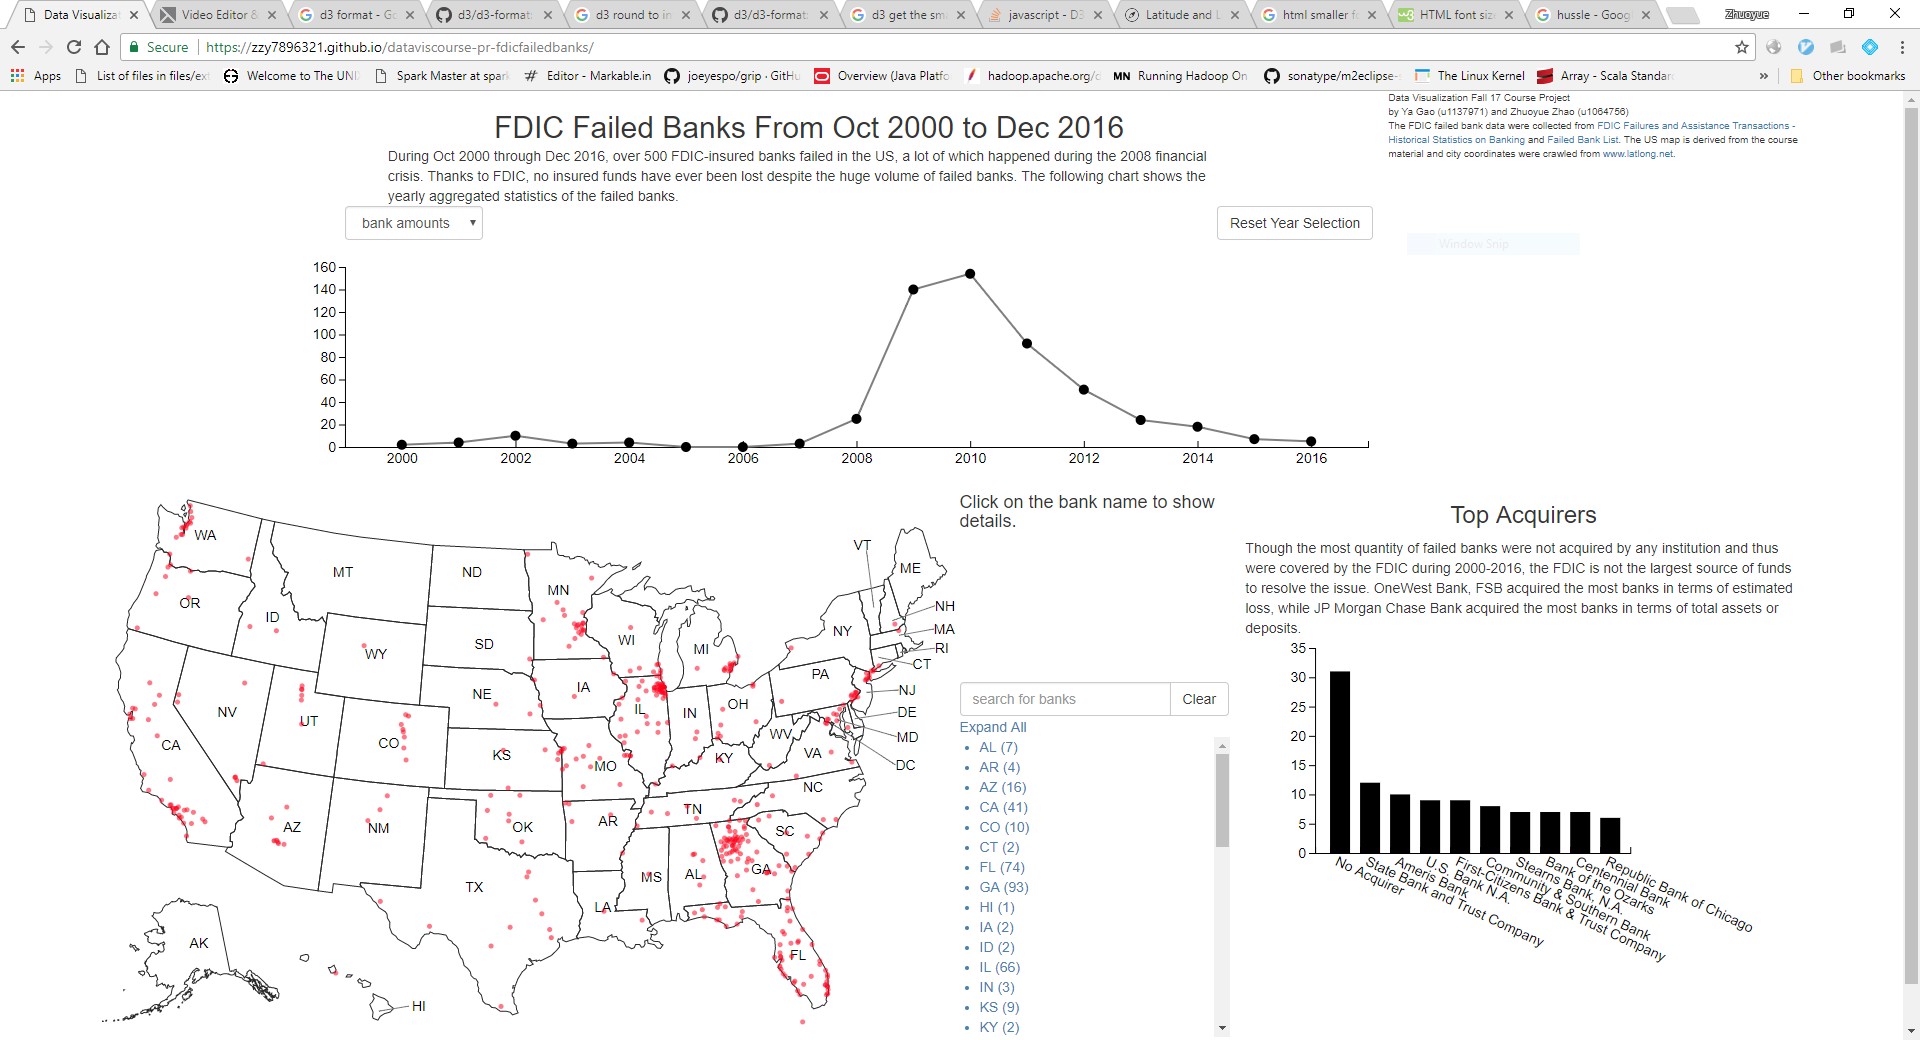
\includegraphics[width=\textwidth]{fig/final}
    \caption{The final visualization}
    \label{fig:final}
\end{figure}

To sum up, Figure~\ref{fig:final} shows our final visualization of the FDIC
failed banks. In addition to d3 and svg for plotting charts, we used bootstrap
to improve the layouts. 

The main view, the line chart, is placed right below the title and a short
introduction to the project. This is the place that a user might first look
at. Then the map and the bar chart are placed side by side below the main
view. When the user starts clicking on the years, he/she can immediately
notice the linked changes below. When further selections are made on the map
and/or the search box, the bar chart continues changes. We also included a
short text below the title of the bar chart to give a hint of the story we
want to tell.

We learnt a lot from the projects about how to design different visualizations
to show different aspects of our data. We also have a better understanding in
the d3 library.

As of the time we submit this work, the website is hosted on Github at
\url{https://zzy7896321.github.io/dataviscourse-pr-fdicfailedbanks/}.


